\documentclass[conference]{IEEEtran}

\usepackage[utf8]{inputenc}
\usepackage{amsmath,amssymb}
\usepackage{array}
\usepackage{booktabs,siunitx}
\usepackage{graphicx}
\usepackage{url}

\begin{document}

\title{How these robustness characteristics scale}

\author{
    \IEEEauthorblockN{Florian Suess}
}

\maketitle

\begin{abstract}
With the main work done so far\footnote{\url{https://github.com/suessflorian/biological-neurons/}} showcasing evidence of some generally favourable robustness characteristics of our ParaLIF activation within LeNet style architectures, it is important to stress that these results are drawn from behaviour on simpler single colour channel datasets MNIST, KMNIST, SVHN and fashionMNIST. In the world of VisionTransformers and the "tried and true" ResNet architectures, we'd like to also enquire how ParaLIF adoption in these more relatable architectures perform within the context of more difficult three channel image datasets like CIFAR-10/100 to get a sense of how these characteristics scale, and at what cost.

\end{abstract}

\begin{IEEEkeywords}
ResNet, ViT, ParaLIF, LIF, CIFAR-10, CIFAR-100, Advaserial Robustness, DeepFool Attack, Fast Gradient Sign Method Attack, Square Attack
\end{IEEEkeywords}

\section{Introduction}
As we have seen, direct training methodologies for S-NN's remain in it\'s infancy. With common approaches typically requiring backpropogation through time methods that unroll potentially an entire network linearly to the number of steps you use for a spike encoding of an input, this leads us to exceedingly longer training times per dataset. ParaLIF, our focus and variant of the leaky integrate and fire neuron (LIF), addresses this shortcoming of S-NN's by selling us the idea that we can backpropogate through time \emph{in parallel} - but as we've seen this hasn't prevented the difficulty associated to training these networks even on small models (~60k parameters).

One could speculate that this issue broadly steps parallel to issues faced by the training of traditional recurrent networks, albeit in the case of S-NN's, we face these issues without the mechanisms such as the LSTM and GRU gradient preserving gates. In spirit of our original research objective, we pivoted early on to \emph{hybrid} models, that is, where typical continuous network features like convolutions could be adopted in front of ParaLIF networks. This is considered a slight concession as pure S-NN models have been shown to have significant potential to exceed in terms of energy efficiency and speed\footnote{cite}. In writing that, hybrid networks still remain valuable to enquire into though as the potential gains of adversarial robustness of networks remains a separate and important objective of any network.

\pagebreak

We have previously in our journey to break our performance boundaries found ANN-SNN conversions effective\footnote{Available here; https://github.com/suessflorian/qcfs/}. We specifically adapted methods published in the literature specific to ResNets. This involved priming techniques (concretely, that is, swapping all ReLU's with "quantised clip-floor shifted" ReLU) such that a recursive activation swap with LIF had a zero conversion error loss. However we deemed this method a bit too restrictive to continue with - predominately because although mapping to LIF based networks was clear, a mapping to ParaLIF activations remained unclear. With the little time we had, we picked out what worked well.

\section{Adoption of ParaLIF in ResNet Models}
The key idea here is to use a ResNets as an encoder of our input up to the point of exit from the final residual layer, decoding this feature map using a single ParaLIF or LIF feed forward linear layer. We batch min max normalise the feature map values into the range $p \in [0,1]$. We use this to "rate encode" this over 20 steps using the same Bernoulli distribution method used throughout this research project. Each step assuming 1 with probability $p$ and 0 with probability 1-$p$. We semi-arbitrarily choose the ResNet models 18 and 50 due to their ubiquitous names as benchmarks.

\subsection{Transfer Learning}
To boost learning time we adopt what we learnt previously and adopt conversion tactics. We fine-tune these ResNets onto CIFAR-10/100. Leveraging the speed up boost by transferring pre-trained weights from heavily trained ResNets on the ImageNet. At the time of this enquiry, we had some readily available (and verifiable) performance characteristics on ImageNet of the following;

\vspace{0.5cm}
\begin{table}[ht]
\centering
\begin{tabular}{ l l l }
  \toprule
  Model & \multicolumn{1}{c}{Accuracy \%} & \multicolumn{1}{c}{Parameters (M)} \\
  \midrule
  ResNet-18 & \num{69.76} & \num{11.7} \\
  ResNet-50 & \num{80.86} & \num{25.6} \\
  \bottomrule
\end{tabular}
\end{table}

\pagebreak

Fine-tuning via training the full network is prone to destructive learning, especially to those low level feature layers - and so we experimented with freezing early residual layers, found that freezing all parameters pre layer 3 was effective.

We didn't have too much time to experiment much with all the various available meta learning hyper parameters but we found the classic SGD optimization method was sufficient, with a low $\eta=0.001$, basic L2 weight regularisation with some training speed increases too with introduced momentum during descent (0.9).

We found more training speed gains by stabilising the 4th residual layer using the default ResNet configuration before transferring to ParaLIF and LIF activations - and so we have indeed demonstrated some sort of \emph{double} learning transfer approach despite our issue of very limited compute.

\section{Test Performance Measure}
\begin{figure}[h!]
    \centering
    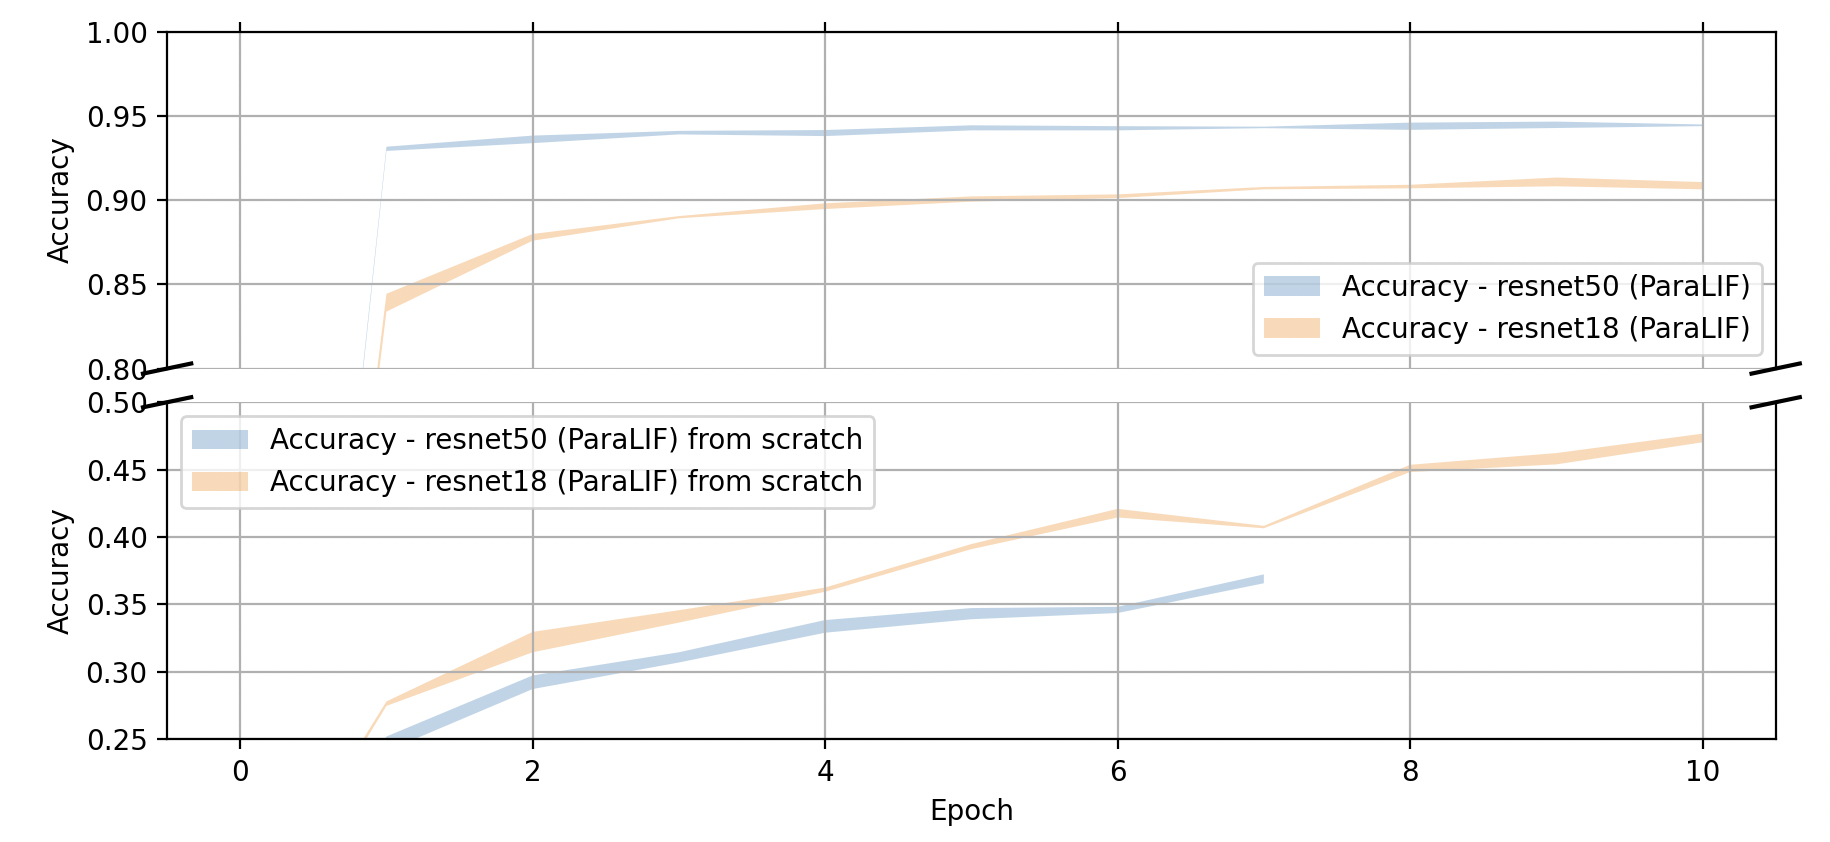
\includegraphics[width=\linewidth]{transfer-contrast.png}
    \caption{The double transfer method test accuracy climbing quickly relative to scratch training}
    \label{fig:transfer_contrast}
\end{figure}

With all of this careful planning, on execution - we quickly surpass previous model performance by significant margin. Allowing for deeper enquiry into CIFAR-10 with a comfortable dataset beat allowing us to start paying attention to CIFAR-100. Although both LIF and ParaLIF contain a stochastic element in their inference (the Bernoulli distribution rate encoding method), we found notable variance in inference outcomes given a fixed image on different random seeds - hence we accompany test results with standard deviation.

\begin{itemize}
    \item All default variants are trained for 10 epochs.
    \item ParaLIF/LIF variants are trained for 10 epochs, with transferred weights of a fine-tuned 4th residual layer from the above.
\end{itemize}

\pagebreak

\begin{table}[ht]
\centering
\begin{tabular}{ l l l }
  FashionMNIST \\
  \\
  Variant & \multicolumn{1}{c}{ResNet-18} & \multicolumn{1}{c}{ResNet-50} \\
  \midrule
  Default & \num{93.2} & \num{93.2} \\
  LIF & \num{93.7} & \num{93.4} \\
  ParaLIF & $91.5\% \pm 0.08\%$ & $92.5\% \pm 0.14\%$ \\
  \bottomrule
\end{tabular}
\end{table}

\begin{table}[ht]
\centering
\begin{tabular}{ l l l }
  CIFAR-10 \\
  \\
  Variant & \multicolumn{1}{c}{ResNet-18\%} & \multicolumn{1}{c}{ResNet-50} \\
  \midrule
  Default & \num{92.4} & \num{94.7} \\
  LIF & \num{92.8} & \num{94.8} \\
  ParaLIF & $90.9\% \pm 0.15\%$ & $94.4\% \pm 0.034\%$ \\
  \bottomrule
\end{tabular}
\end{table}

\begin{table}[ht]
\centering
\begin{tabular}{ l l l }
  CIFAR-100 \\
  \\
  Variant & \multicolumn{1}{c}{ResNet-18 \%} & \multicolumn{1}{c}{ResNet-50} \\
  \midrule
  Default & \num{73.3} & \num{77.9} \\
  LIF & \num{74.3} & \num{79.4} \\
  ParaLIF & $34.9\% \pm 0.08\%$ & $52.9\% \pm 0.14\%$ \\
  \bottomrule
\end{tabular}
\end{table}

\section{Attacks}
We proceed from here to start attacking these models with same attacks our earlier endeavours, particularly measuring contrastive performance wrt. each dataset and model.

\subsection*{Fast Gradient Sign Method Attack}

\begin{figure}[h!]
    \centering
    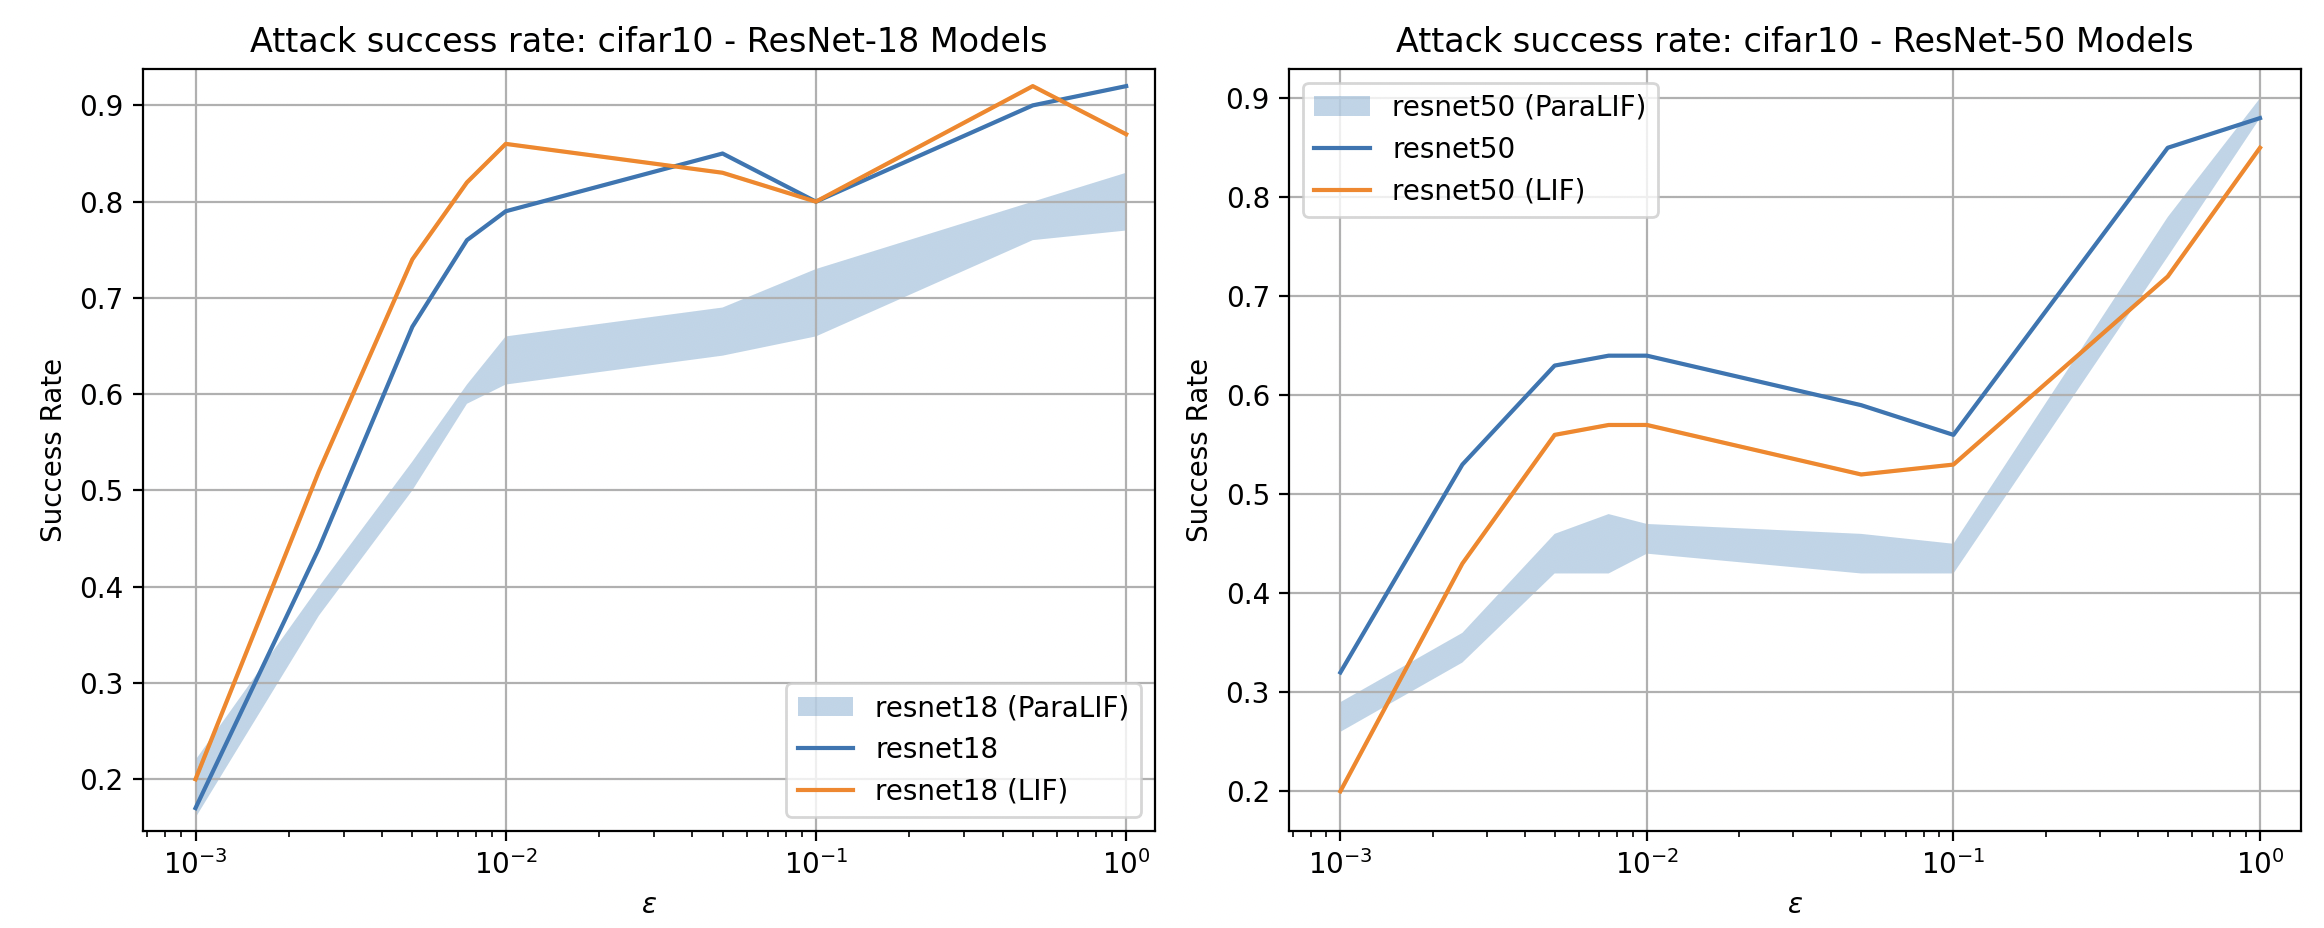
\includegraphics[width=\linewidth]{resnet-fgsm-cifar10.png}
    \caption{FGSM attack at various epsilons}
    \label{fig:resnet_fgsm_attack}
\end{figure}

\subsection*{DeepFool Attack}

\begin{figure}[h!]
    \centering
    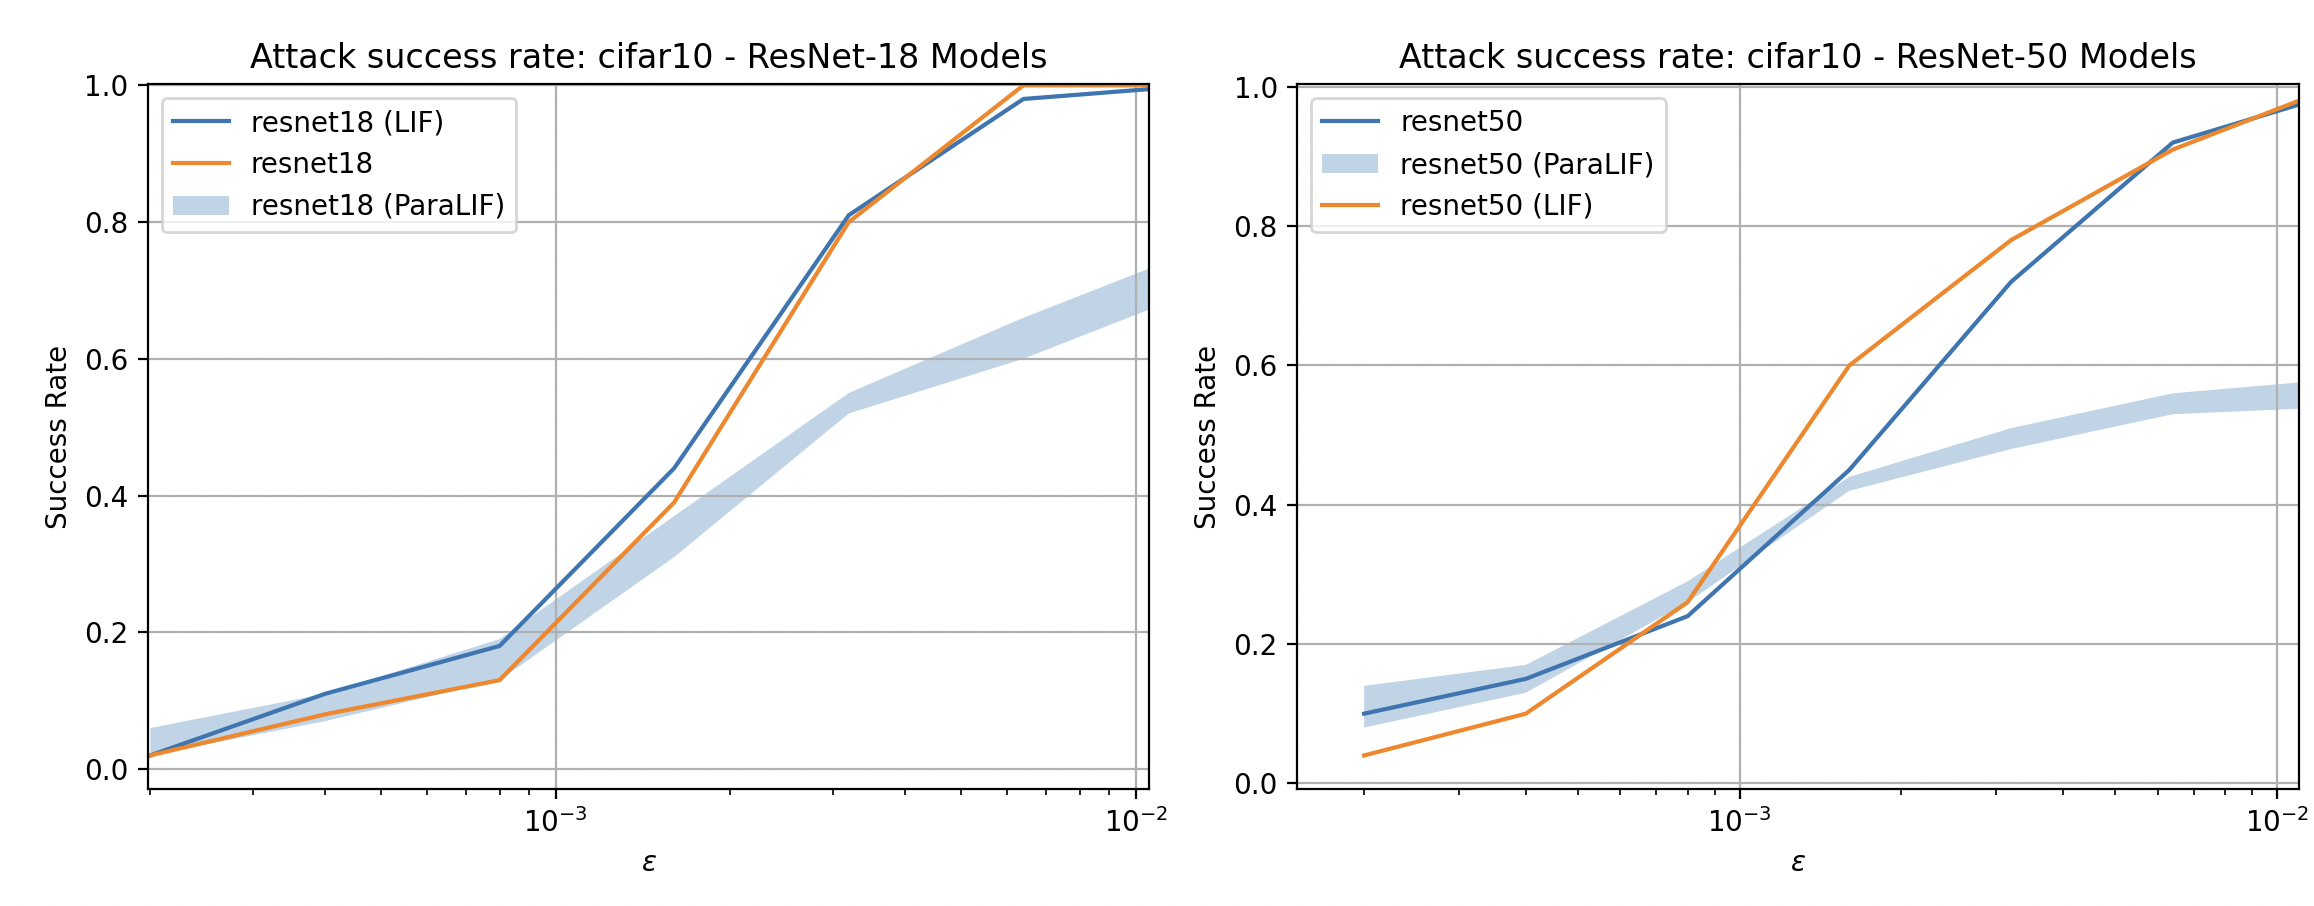
\includegraphics[width=\linewidth]{resnet-deepfool-cifar10.png}
    \caption{Deepfool attack at a fixed max iterations of 100 at various epsilons}
    \label{fig:resnet_deepfool_attack}
\end{figure}

\pagebreak

\subsection*{Square Attack}

\begin{figure}[h!]
    \centering
    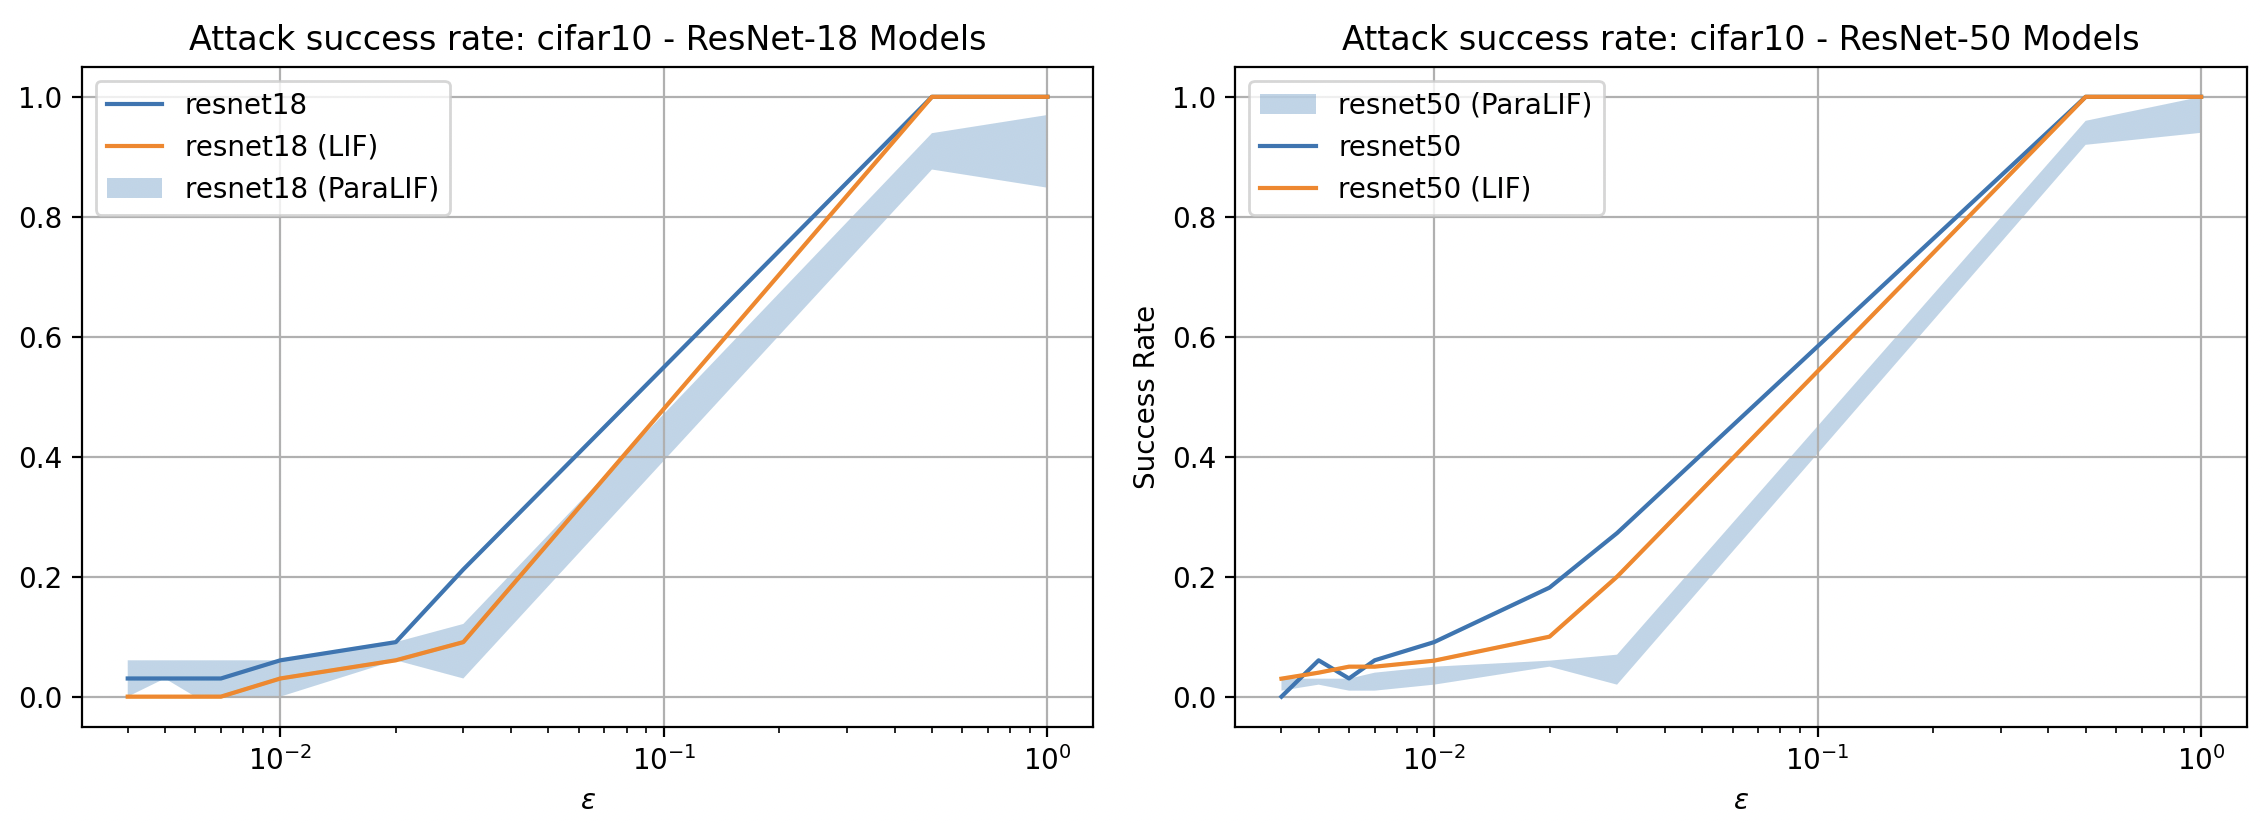
\includegraphics[width=\linewidth]{resnet-square-cifar10.png}
    \caption{Square attack at a fixed max iterations of 100 at various epsilons}
    \label{fig:resnet_square_attack}
\end{figure}

\section{Adoption of ParaLIF in Vision Transformer Models}
ResNets as an encoder of our input up to the point of exit from the final residual layer, decoding this feature map using a single ParaLIF or LIF feed forward linear layer. We batch min max normalise the feature map values into the range $p \in [0,1]$. We use this to "rate encode" this over 20 steps using the same Bernoulli distribution method used throughout this research project. Each step assuming 1 with probability $p$ and 0 with probability 1-$p$. We semi-arbitrarily choose the ResNet models 18 and 50 due to their ubiquitous names as benchmarks.

\section{TradeOff}
Although we see various robustness characteristics in ParaLIF based networks.... TODO

\begin{figure}[h!]
    \centering
    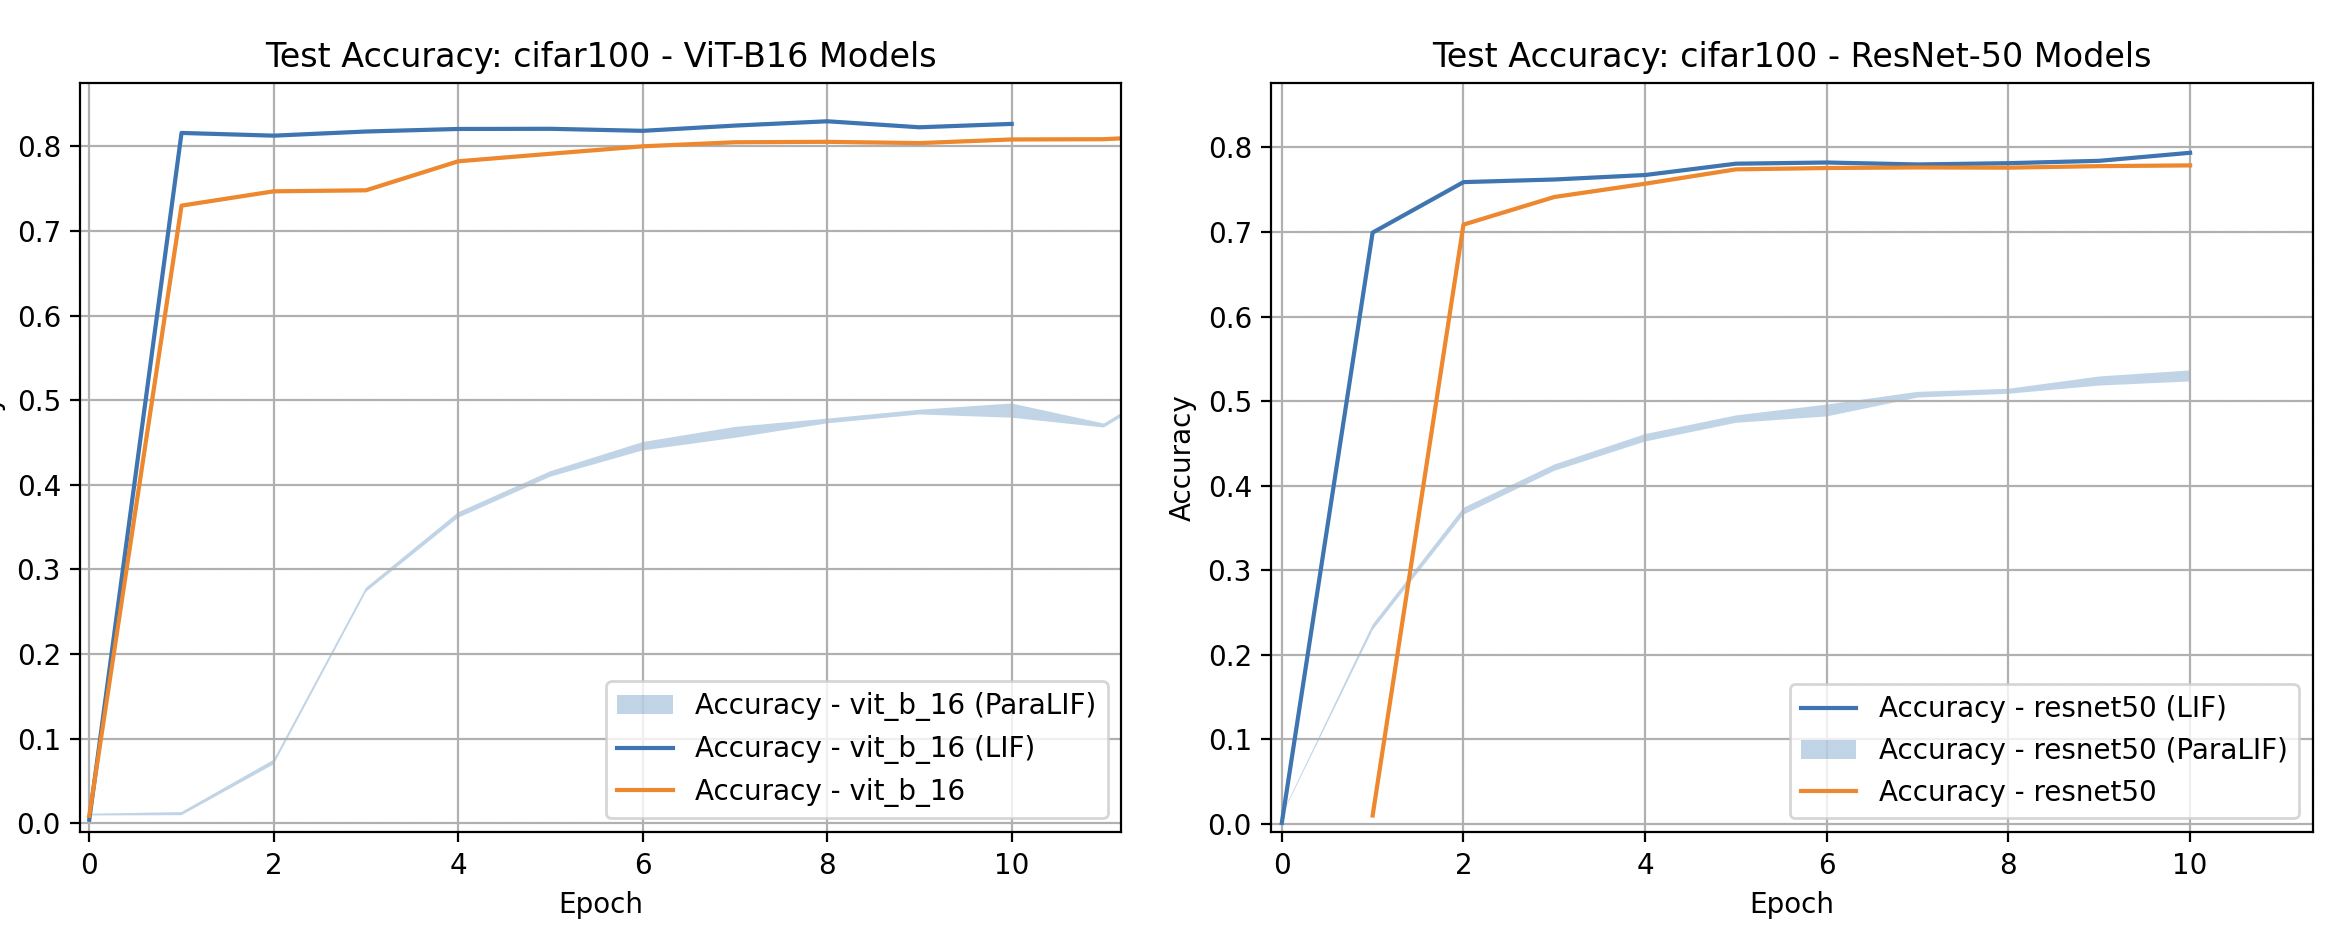
\includegraphics[width=\linewidth]{resnet-transformer-cifar100.png}
    \caption{Transformer and ResNet ParaLIF models struggling to learn on CIFAR-100}
    \label{fig:resnet_transformer_cifar100}
\end{figure}


\end{document}
